\documentclass[11pt,a4paper]{article}
\usepackage[utf8]{inputenc}
\usepackage[margin=2.5cm]{geometry}
\usepackage{amsmath,amssymb,amsfonts}
\usepackage{graphicx}

\setlength{\parindent}{0pt}
\setlength{\parskip}{6pt}

\begin{document}

% --- Header Identitas Tugas ---
\begin{center}
    {\large \textbf{TUGAS 1 MA4171 TEORI KONTROL LINEAR}}\\[4pt]
    \textbf{Nama:} \underline{\hspace{5cm}} \qquad \textbf{NIM:} \underline{\hspace{3.5cm}}
\end{center}
\vspace{-4pt}
\hrule
\vspace{12pt}

% --- Soal dan Pembahasan Nomor 1 ---
\setcounter{equation}{0}
\noindent \textbf{1. Tentukan solusi dari masalah nilai awal berikut dengan menggunakan transformasi Laplace:}

\vspace{6pt}
\setcounter{equation}{0}
\noindent \textbf{(a)} $y'' - 2y' + y = \cos(t), \quad y(0) = 1, \quad y'(0) = 0$

\vspace{2pt}
\noindent \textit{Penyelesaian:}

Terapkan transformasi Laplace pada kedua ruas persamaan:
\begin{align*}
    \mathcal{L}\{y'' - 2y' + y\} &= \mathcal{L}\{\cos(t)\} \\
    \mathcal{L}\{y''\} - 2\mathcal{L}\{y'\} + \mathcal{L}\{y\} &= \frac{s}{s^2 + 1}
\end{align*}

Gunakan sifat turunan transformasi Laplace:
\begin{align*}
    \mathcal{L}\{y'\} &= sY(s) - y(0) = sY(s) - 1 \\
    \mathcal{L}\{y''\} &= s^2Y(s) - sy(0) - y'(0) = s^2Y(s) - s(1) - 0 = s^2Y(s) - s
\end{align*}

Substitusikan ke dalam persamaan diferensial:
\begin{align*}
    (s^2Y(s) - s) - 2(sY(s) - 1) + Y(s) &= \frac{s}{s^2 + 1} \\
    (s^2 - 2s + 1)Y(s) - s + 2 &= \frac{s}{s^2 + 1} \\
    (s - 1)^2 Y(s) &= s - 2 + \frac{s}{s^2 + 1}
\end{align*}

Sederhanakan ruas kanan untuk memperoleh bentuk aljabar $Y(s)$:
\begin{align*}
    (s - 1)^2 Y(s) &= \frac{(s - 2)(s^2 + 1) + s}{s^2 + 1} \\
    (s - 1)^2 Y(s) &= \frac{s^3 - 2s^2 + 2s - 2}{s^2 + 1} \\
    Y(s) &= \frac{s^3 - 2s^2 + 2s - 2}{(s - 1)^2(s^2 + 1)}
\end{align*}

Lakukan dekomposisi pecahan parsial:
\begin{equation*}
    \frac{s^3 - 2s^2 + 2s - 2}{(s - 1)^2(s^2 + 1)} = \frac{A}{s - 1} + \frac{B}{(s - 1)^2} + \frac{Cs + D}{s^2 + 1}
\end{equation*}

Kalikan kedua ruas dengan $(s - 1)^2(s^2 + 1)$:
\begin{equation*}
    s^3 - 2s^2 + 2s - 2 = A(s - 1)(s^2 + 1) + B(s^2 + 1) + (Cs + D)(s - 1)^2
\end{equation*}

Substitusi $s = 1$ untuk mencari $B$:
\begin{align*}
    1^3 - 2(1)^2 + 2(1) - 2 &= B(1^2 + 1) \\
    -1 &= 2B \implies B = -\frac{1}{2}
\end{align*}

Jabarkan ruas kanan dan samakan koefisiennya:
\begin{align*}
    s^3 - 2s^2 + 2s - 2 &= (A + C)s^3 + (-A + B - 2C + D)s^2 + (A + C - 2D)s + (-A + B + D)
\end{align*}

Dari kesamaan koefisien:
\begin{align*}
    \text{Koefisien } s^3 &: A + C = 1 \\
    \text{Koefisien } s &: (A + C) - 2D = 2 \implies 1 - 2D = 2 \implies D = -\frac{1}{2} \\
    \text{Konstanta} &: -A + B + D = -2 \implies -A - \frac{1}{2} - \frac{1}{2} = -2 \implies A = 1 \\
    \text{Nilai } C &: C = 1 - A = 1 - 1 = 0
\end{align*}

Sehingga $Y(s)$ dapat dituliskan sebagai:
\begin{equation*}
    Y(s) = \frac{1}{s - 1} - \frac{1}{2}\frac{1}{(s - 1)^2} - \frac{1}{2}\frac{1}{s^2 + 1}
\end{equation*}

Terapkan invers transformasi Laplace:
\begin{align*}
    \mathcal{L}^{-1}\left\{\frac{1}{s - 1}\right\} &= e^t \\
    \mathcal{L}^{-1}\left\{\frac{1}{(s - 1)^2}\right\} &= t e^t \\
    \mathcal{L}^{-1}\left\{\frac{1}{s^2 + 1}\right\} &= \sin(t)
\end{align*}

Diperoleh solusi:
\begin{equation*}
    y(t) = e^t - \frac{1}{2}t e^t - \frac{1}{2}\sin(t)
\end{equation*}

\vspace{16pt}

% --- Nomor 1 (b) ---
\setcounter{equation}{0}
\noindent \textbf{(b)} $y'' + 2y' + y = 4e^{-t}, \quad y(0) = 2, \quad y'(0) = -1$

\vspace{2pt}
\noindent \textit{Penyelesaian:}

Terapkan transformasi Laplace pada kedua ruas persamaan:
\begin{align*}
    \mathcal{L}\{y'' + 2y' + y\} &= \mathcal{L}\{4e^{-t}\} \\
    \mathcal{L}\{y''\} + 2\mathcal{L}\{y'\} + \mathcal{L}\{y\} &= \frac{4}{s + 1}
\end{align*}

Gunakan sifat turunan transformasi Laplace dan kondisi awal:
\begin{align*}
    \mathcal{L}\{y'\} &= sY(s) - y(0) = sY(s) - 2 \\
    \mathcal{L}\{y''\} &= s^2Y(s) - sy(0) - y'(0) = s^2Y(s) - 2s - (-1) = s^2Y(s) - 2s + 1
\end{align*}

Substitusikan ke dalam persamaan diferensial:
\begin{align*}
    (s^2Y(s) - 2s + 1) + 2(sY(s) - 2) + Y(s) &= \frac{4}{s + 1} \\
    (s^2 + 2s + 1)Y(s) - 2s - 3 &= \frac{4}{s + 1} \\
    (s + 1)^2 Y(s) &= 2s + 3 + \frac{4}{s + 1}
\end{align*}

Bagi kedua ruas dengan $(s + 1)^2$ dan lakukan dekomposisi pecahan parsial:
\begin{align*}
    Y(s) &= \frac{2s + 3}{(s + 1)^2} + \frac{4}{(s + 1)^3} \\
    &= \frac{2(s + 1) + 1}{(s + 1)^2} + \frac{4}{(s + 1)^3} \\
    &= \frac{2}{s + 1} + \frac{1}{(s + 1)^2} + \frac{4}{(s + 1)^3}
\end{align*}

Terapkan invers transformasi Laplace:
\begin{align*}
    \mathcal{L}^{-1}\left\{\frac{1}{s + 1}\right\} &= e^{-t} \\
    \mathcal{L}^{-1}\left\{\frac{1}{(s + 1)^2}\right\} &= t e^{-t} \\
    \mathcal{L}^{-1}\left\{\frac{4}{(s + 1)^3}\right\} &= 4 \left(\frac{1}{2!}t^2 e^{-t}\right) = 2t^2 e^{-t}
\end{align*}

Diperoleh solusi:
\begin{align*}
    y(t) &= 2e^{-t} + t e^{-t} + 2t^2 e^{-t} \\
    y(t) &= (2 + t + 2t^2) e^{-t}
\end{align*}

\vspace{18pt}

% --- Soal dan Pembahasan Nomor 2 ---
\setcounter{equation}{0}
\noindent \textbf{2. Carilah persamaan ruang keadaan sistem $y''' + 2y'' - 3y' + 6y = 10u$ dalam bentuk:}
\begin{equation*}
    \begin{cases}
        \mathbf{\dot{x}} = A\mathbf{x} + Bu \\
        y = C\mathbf{x} + Du
    \end{cases}
\end{equation*}
\textbf{kemudian dari persamaan ruang keadaan tersebut, tentukan fungsi transfernya.}

\vspace{2pt}
\noindent \textit{Penyelesaian:}

Tuliskan turunan tertinggi pada ruas kiri:
\begin{equation*}
    y''' = -6y + 3y' - 2y'' + 10u
\end{equation*}

Definisikan variabel keadaan sebagai berikut:
\begin{align*}
    x_1 &= y \\
    x_2 &= y' = \dot{x}_1 \\
    x_3 &= y'' = \dot{x}_2
\end{align*}

Turunan dari masing-masing variabel keadaan adalah:
\begin{align*}
    \dot{x}_1 &= x_2 \\
    \dot{x}_2 &= x_3 \\
    \dot{x}_3 &= y''' = -6x_1 + 3x_2 - 2x_3 + 10u
\end{align*}

Susun persamaan keadaan dan persamaan keluaran dalam bentuk matriks:
\begin{align*}
    \begin{bmatrix}
        \dot{x}_1 \\ \dot{x}_2 \\ \dot{x}_3
    \end{bmatrix}
    &=
    \begin{bmatrix}
        0 & 1 & 0 \\
        0 & 0 & 1 \\
        -6 & 3 & -2
    \end{bmatrix}
    \begin{bmatrix}
        x_1 \\ x_2 \\ x_3
    \end{bmatrix}
    +
    \begin{bmatrix}
        0 \\ 0 \\ 10
    \end{bmatrix}
    u \\[6pt]
    y &=
    \begin{bmatrix}
        1 & 0 & 0
    \end{bmatrix}
    \begin{bmatrix}
        x_1 \\ x_2 \\ x_3
    \end{bmatrix}
    +
    [0]u
\end{align*}

Sehingga matriks representasi ruang keadaan diperoleh:
\begin{equation*}
    A = \begin{bmatrix} 0 & 1 & 0 \\ 0 & 0 & 1 \\ -6 & 3 & -2 \end{bmatrix}, \quad
    B = \begin{bmatrix} 0 \\ 0 \\ 10 \end{bmatrix}, \quad
    C = \begin{bmatrix} 1 & 0 & 0 \end{bmatrix}, \quad
    D = 0
\end{equation*}

Selanjutnya, tentukan fungsi transfer menggunakan rumus:
\begin{equation*}
    G(s) = \frac{Y(s)}{U(s)} = C(sI - A)^{-1}B + D
\end{equation*}

Bentuk matriks $(sI - A)$:
\begin{equation*}
    sI - A =
    s \begin{bmatrix} 1 & 0 & 0 \\ 0 & 1 & 0 \\ 0 & 0 & 1 \end{bmatrix}
    -
    \begin{bmatrix} 0 & 1 & 0 \\ 0 & 0 & 1 \\ -6 & 3 & -2 \end{bmatrix}
    =
    \begin{bmatrix}
        s & -1 & 0 \\
        0 & s & -1 \\
        6 & -3 & s + 2
    \end{bmatrix}
\end{equation*}

Hitung determinan dari $(sI - A)$:
\begin{align*}
    \det(sI - A) &= s \begin{vmatrix} s & -1 \\ -3 & s + 2 \end{vmatrix} - (-1)\begin{vmatrix} 0 & -1 \\ 6 & s + 2 \end{vmatrix} + 0 \\
    &= s(s(s + 2) - 3) + 1(0 - (-6)) \\
    &= s(s^2 + 2s - 3) + 6 \\
    &= s^3 + 2s^2 - 3s + 6
\end{align*}

Tentukan invers matriks $(sI - A)^{-1} = \frac{1}{\det(sI - A)}\operatorname{adj}(sI - A)$. Karena $C = \begin{bmatrix} 1 & 0 & 0 \end{bmatrix}$, maka baris pertama dari $(sI - A)^{-1}$ diperoleh dari kofaktor baris pertama adjoin (kofaktor kolom pertama dari $sI - A$):
\begin{align*}
    C_{11} &= + \begin{vmatrix} s & -1 \\ -3 & s + 2 \end{vmatrix} = s^2 + 2s - 3 \\
    C_{21} &= - \begin{vmatrix} -1 & 0 \\ -3 & s + 2 \end{vmatrix} = -(-s - 2) = s + 2 \\
    C_{31} &= + \begin{vmatrix} -1 & 0 \\ s & -1 \end{vmatrix} = 1 - 0 = 1
\end{align*}

Sehingga baris pertama dari $(sI - A)^{-1}$ adalah:
\begin{equation*}
    C(sI - A)^{-1} = \frac{1}{s^3 + 2s^2 - 3s + 6}\begin{bmatrix} s^2 + 2s - 3 & s + 2 & 1 \end{bmatrix}
\end{equation*}

Kalikan dengan matriks $B$:
\begin{align*}
    G(s) &= C(sI - A)^{-1}B + 0 \\
    &= \frac{1}{s^3 + 2s^2 - 3s + 6}
    \begin{bmatrix} s^2 + 2s - 3 & s + 2 & 1 \end{bmatrix}
    \begin{bmatrix} 0 \\ 0 \\ 10 \end{bmatrix} \\
    &= \frac{10}{s^3 + 2s^2 - 3s + 6}
\end{align*}

Diperoleh fungsi transfer sistem:
\begin{equation*}
    G(s) = \frac{Y(s)}{U(s)} = \frac{10}{s^3 + 2s^2 - 3s + 6}
\end{equation*}

\vspace{18pt}

% --- Soal dan Pembahasan Nomor 3 ---
\setcounter{equation}{0}
\noindent \textbf{3. Tentukan fungsi transfer kemudian sederhanakanlah diagram blok sistem berikut.}

\begin{center}
    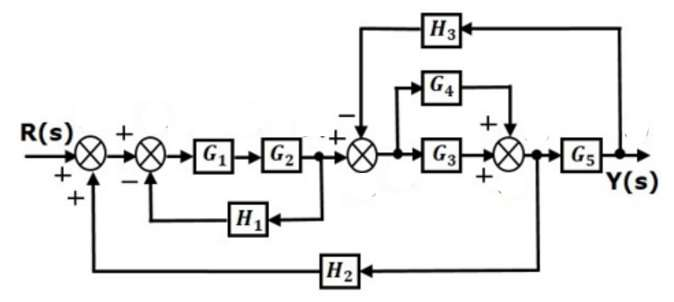
\includegraphics[width=0.72\textwidth]{problem_img_3.jpg}
\end{center}

\vspace{2pt}
\noindent \textit{Penyelesaian:}

Untuk mempermudah penentuan fungsi transfer sistem, kita definisikan terlebih dahulu nama sinyal pada setiap simpul diagram blok:
\begin{itemize}
    \item $R(s)$: Sinyal masukan referensi utama.
    \item $Y(s)$: Sinyal keluaran sistem.
    \item $E_1(s)$: Sinyal setelah titik penjumlahan pertama.
    \item $E_2(s)$: Sinyal masukan ke blok $G_1$ (setelah titik penjumlahan kedua).
    \item $X_1(s)$: Sinyal keluaran setelah blok seri $G_1$ dan $G_2$.
    \item $X_2(s)$: Sinyal setelah titik penjumlahan ketiga.
    \item $X_3(s)$: Sinyal keluaran setelah penjumlahan cabang paralel $G_3$ dan $G_4$.
\end{itemize}

Berdasarkan diagram blok, kita susun persamaan pada masing-masing simpul:

Tinjau titik penjumlahan kedua dan blok kaskade $G_1, G_2$:
\begin{equation}
    \label{eq:e2}
    E_2(s) = E_1(s) - H_1 X_1(s)
\end{equation}
\begin{equation}
    \label{eq:x1_raw}
    X_1(s) = G_1 G_2 E_2(s)
\end{equation}

Substitusikan \eqref{eq:e2} ke dalam \eqref{eq:x1_raw}:
\begin{align*}
    X_1(s) &= G_1 G_2 \left[ E_1(s) - H_1 X_1(s) \right] \\
    X_1(s) + G_1 G_2 H_1 X_1(s) &= G_1 G_2 E_1(s) \\
    (1 + G_1 G_2 H_1) X_1(s) &= G_1 G_2 E_1(s)
\end{align*}
sehingga diperoleh:
\begin{equation}
    \label{eq:x1}
    X_1(s) = G_A E_1(s), \quad \text{dengan } G_A = \frac{G_1 G_2}{1 + G_1 G_2 H_1}
\end{equation}

Tinjau titik penjumlahan ketiga:
\begin{equation}
    \label{eq:x2}
    X_2(s) = X_1(s) - H_3 Y(s)
\end{equation}

Tinjau penjumlahan dua jalur paralel $G_3$ dan $G_4$:
\begin{equation}
    \label{eq:x3}
    X_3(s) = (G_3 + G_4) X_2(s)
\end{equation}

Tinjau blok $G_5$ dan keluaran $Y(s)$:
\begin{equation}
    \label{eq:y}
    Y(s) = G_5 X_3(s) \implies X_3(s) = \frac{Y(s)}{G_5}
\end{equation}

Tinjau titik penjumlahan pertama:
\begin{equation}
    \label{eq:e1}
    E_1(s) = R(s) + H_2 X_3(s)
\end{equation}

Selanjutnya, lakukan eliminasi terhadap sinyal-sinyal perantara dengan substitusi bertahap:

Substitusikan \eqref{eq:x2} ke dalam \eqref{eq:x3}:
\begin{equation*}
    X_3(s) = (G_3 + G_4) \left[ X_1(s) - H_3 Y(s) \right]
\end{equation*}

Substitusikan \eqref{eq:x1} ke dalam persamaan di atas:
\begin{equation*}
    X_3(s) = (G_3 + G_4) \left[ G_A E_1(s) - H_3 Y(s) \right]
\end{equation*}

Substitusikan \eqref{eq:e1} ke dalam persamaan di atas:
\begin{equation*}
    X_3(s) = (G_3 + G_4) \left[ G_A \left( R(s) + H_2 X_3(s) \right) - H_3 Y(s) \right]
\end{equation*}

Gunakan hubungan $X_3(s)$ dari \eqref{eq:y}:
\begin{equation*}
    \frac{Y(s)}{G_5} = (G_3 + G_4) \left[ G_A R(s) + G_A H_2 \frac{Y(s)}{G_5} - H_3 Y(s) \right]
\end{equation*}

Kalikan kedua ruas dengan $G_5$:
\begin{equation*}
    Y(s) = G_A G_5 (G_3 + G_4) R(s) + G_A (G_3 + G_4) H_2 Y(s) - G_5 (G_3 + G_4) H_3 Y(s)
\end{equation*}

Kumpulkan seluruh suku yang memuat $Y(s)$ ke ruas kiri:
\begin{align*}
    Y(s) - G_A (G_3 + G_4) H_2 Y(s) + G_5 (G_3 + G_4) H_3 Y(s) &= G_A G_5 (G_3 + G_4) R(s) \\
    \left[ 1 - G_A (G_3 + G_4) H_2 + G_5 (G_3 + G_4) H_3 \right] Y(s) &= G_A G_5 (G_3 + G_4) R(s)
\end{align*}

Bagi kedua ruas untuk memperoleh fungsi transfer $\dfrac{Y(s)}{R(s)}$:
\begin{equation*}
    \frac{Y(s)}{R(s)} = \frac{G_A G_5 (G_3 + G_4)}{1 - G_A (G_3 + G_4) H_2 + G_5 (G_3 + G_4) H_3}
\end{equation*}

Substitusikan nilai $G_A$ dari \eqref{eq:x1}:
\begin{equation*}
    \frac{Y(s)}{R(s)} = \frac{\left( \dfrac{G_1 G_2}{1 + G_1 G_2 H_1} \right) G_5 (G_3 + G_4)}{1 - \left( \dfrac{G_1 G_2}{1 + G_1 G_2 H_1} \right) (G_3 + G_4) H_2 + G_5 (G_3 + G_4) H_3}
\end{equation*}

Kalikan pembilang dan penyebut dengan faktor $(1 + G_1 G_2 H_1)$:
\begin{align*}
    \frac{Y(s)}{R(s)} &= \frac{G_1 G_2 G_5 (G_3 + G_4)}{(1 + G_1 G_2 H_1)\left[ 1 + G_5 (G_3 + G_4) H_3 \right] - G_1 G_2 (G_3 + G_4) H_2}
\end{align*}

Jabarkan penyebut persamaan di atas:
\begin{equation*}
    (1 + G_1 G_2 H_1)\left[ 1 + G_5 (G_3 + G_4) H_3 \right] = 1 + G_1 G_2 H_1 + G_5 (G_3 + G_4) H_3 + G_1 G_2 G_5 H_1 (G_3 + G_4) H_3
\end{equation*}

Sehingga fungsi transfer keseluruhan sistem diperoleh:
\begin{equation*}
    \frac{Y(s)}{R(s)} = \frac{G_1 G_2 G_5 (G_3 + G_4)}{1 + G_1 G_2 H_1 + G_5 (G_3 + G_4) H_3 + G_1 G_2 G_5 H_1 (G_3 + G_4) H_3 - G_1 G_2 (G_3 + G_4) H_2}
\end{equation*}

\vspace{18pt}

% --- Soal dan Pembahasan Nomor 4 ---
\setcounter{equation}{0}
\noindent \textbf{4. Diagram blok suatu sistem diberikan seperti pada gambar berikut. Jika persamaan ruang keadaan dari sistem $G_i$ adalah $\left[ \begin{array}{c|c} A_i & B_i \\ \hline C_i & D_i \end{array} \right]$, tentukan persamaan ruang keadaan dari $u$ ke $y$.}

\begin{center}
    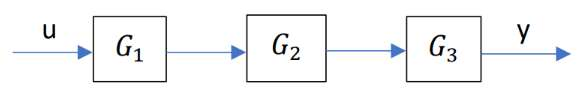
\includegraphics[width=0.72\textwidth]{problem_img_4.jpg}
\end{center}

\vspace{2pt}
\noindent \textit{Penyelesaian:}

Berdasarkan diagram blok di atas, sistem tersusun dari tiga subsistem $G_1$, $G_2$, dan $G_3$ yang terhubung secara seri (kaskade). Untuk masing-masing subsistem $G_i$ ($i = 1, 2, 3$), persamaan ruang keadaan dengan vektor keadaan $\mathbf{x}_i$, sinyal masukan $u_i$, dan sinyal keluaran $y_i$ dinyatakan oleh:
\begin{align*}
    \mathbf{\dot{x}}_i &= A_i \mathbf{x}_i + B_i u_i \\
    y_i &= C_i \mathbf{x}_i + D_i u_i
\end{align*}

Tuliskan persamaan keadaan dan keluaran untuk masing-masing subsistem:

Untuk subsistem $G_1$, sinyal masukannya adalah masukan utama sistem, yaitu $u_1 = u$:
\begin{equation}
    \label{eq:g1_state}
    \mathbf{\dot{x}}_1 = A_1 \mathbf{x}_1 + B_1 u
\end{equation}
\begin{equation}
    \label{eq:g1_out}
    y_1 = C_1 \mathbf{x}_1 + D_1 u
\end{equation}

Untuk subsistem $G_2$, sinyal masukannya adalah keluaran dari subsistem pertama, yaitu $u_2 = y_1$:
\begin{equation}
    \label{eq:g2_state}
    \mathbf{\dot{x}}_2 = A_2 \mathbf{x}_2 + B_2 u_2
\end{equation}
\begin{equation}
    \label{eq:g2_out}
    y_2 = C_2 \mathbf{x}_2 + D_2 u_2
\end{equation}

Untuk subsistem $G_3$, sinyal masukannya adalah keluaran dari subsistem kedua, yaitu $u_3 = y_2$, dan keluarannya adalah keluaran akhir sistem $y = y_3$:
\begin{equation}
    \label{eq:g3_state}
    \mathbf{\dot{x}}_3 = A_3 \mathbf{x}_3 + B_3 u_3
\end{equation}
\begin{equation}
    \label{eq:g3_out}
    y = C_3 \mathbf{x}_3 + D_3 u_3
\end{equation}

Selanjutnya, lakukan substitusi sinyal antarsubsistem ke dalam persamaan keadaan dan keluaran:

Substitusikan $u_2 = y_1$ dari \eqref{eq:g1_out} ke dalam \eqref{eq:g2_state}:
\begin{align}
    \label{eq:x2_dot}
    \mathbf{\dot{x}}_2 &= A_2 \mathbf{x}_2 + B_2 (C_1 \mathbf{x}_1 + D_1 u) \nonumber \\
    \mathbf{\dot{x}}_2 &= B_2 C_1 \mathbf{x}_1 + A_2 \mathbf{x}_2 + B_2 D_1 u
\end{align}

Substitusikan $u_2 = y_1$ dari \eqref{eq:g1_out} ke dalam \eqref{eq:g2_out}:
\begin{align}
    \label{eq:y2}
    y_2 &= C_2 \mathbf{x}_2 + D_2 (C_1 \mathbf{x}_1 + D_1 u) \nonumber \\
    y_2 &= D_2 C_1 \mathbf{x}_1 + C_2 \mathbf{x}_2 + D_2 D_1 u
\end{align}

Substitusikan $u_3 = y_2$ dari \eqref{eq:y2} ke dalam \eqref{eq:g3_state}:
\begin{align}
    \label{eq:x3_dot}
    \mathbf{\dot{x}}_3 &= A_3 \mathbf{x}_3 + B_3 (D_2 C_1 \mathbf{x}_1 + C_2 \mathbf{x}_2 + D_2 D_1 u) \nonumber \\
    \mathbf{\dot{x}}_3 &= B_3 D_2 C_1 \mathbf{x}_1 + B_3 C_2 \mathbf{x}_2 + A_3 \mathbf{x}_3 + B_3 D_2 D_1 u
\end{align}

Substitusikan $u_3 = y_2$ dari \eqref{eq:y2} ke dalam \eqref{eq:g3_out}:
\begin{align}
    \label{eq:y_out}
    y &= C_3 \mathbf{x}_3 + D_3 (D_2 C_1 \mathbf{x}_1 + C_2 \mathbf{x}_2 + D_2 D_1 u) \nonumber \\
    y &= D_3 D_2 C_1 \mathbf{x}_1 + D_3 C_2 \mathbf{x}_2 + C_3 \mathbf{x}_3 + D_3 D_2 D_1 u
\end{align}

Definisikan vektor keadaan gabungan keseluruhan sistem sebagai:
\begin{equation*}
    \mathbf{x} = \begin{bmatrix} \mathbf{x}_1 \\ \mathbf{x}_2 \\ \mathbf{x}_3 \end{bmatrix}
\end{equation*}

Berdasarkan persamaan diferensial keadaan \eqref{eq:g1_state}, \eqref{eq:x2_dot}, dan \eqref{eq:x3_dot}, persamaan keadaan keseluruhan sistem dapat dituliskan dalam bentuk matriks blok:
\begin{equation*}
    \begin{bmatrix}
        \mathbf{\dot{x}}_1 \\
        \mathbf{\dot{x}}_2 \\
        \mathbf{\dot{x}}_3
    \end{bmatrix}
    =
    \begin{bmatrix}
        A_1 & 0 & 0 \\
        B_2 C_1 & A_2 & 0 \\
        B_3 D_2 C_1 & B_3 C_2 & A_3
    \end{bmatrix}
    \begin{bmatrix}
        \mathbf{x}_1 \\
        \mathbf{x}_2 \\
        \mathbf{x}_3
    \end{bmatrix}
    +
    \begin{bmatrix}
        B_1 \\
        B_2 D_1 \\
        B_3 D_2 D_1
    \end{bmatrix}
    u
\end{equation*}

Berdasarkan persamaan keluaran \eqref{eq:y_out}, persamaan keluaran keseluruhan sistem dapat dituliskan sebagai:
\begin{equation*}
    y =
    \begin{bmatrix}
        D_3 D_2 C_1 & D_3 C_2 & C_3
    \end{bmatrix}
    \begin{bmatrix}
        \mathbf{x}_1 \\
        \mathbf{x}_2 \\
        \mathbf{x}_3
    \end{bmatrix}
    +
    \left[ D_3 D_2 D_1 \right] u
\end{equation*}

Sehingga matriks representasi ruang keadaan sistem kaskade dari $u$ ke $y$ diperoleh:
\begin{align*}
    A &= \begin{bmatrix}
        A_1 & 0 & 0 \\
        B_2 C_1 & A_2 & 0 \\
        B_3 D_2 C_1 & B_3 C_2 & A_3
    \end{bmatrix}, \quad
    B = \begin{bmatrix}
        B_1 \\
        B_2 D_1 \\
        B_3 D_2 D_1
    \end{bmatrix} \\[6pt]
    C &= \begin{bmatrix}
        D_3 D_2 C_1 & D_3 C_2 & C_3
    \end{bmatrix}, \quad
    D = D_3 D_2 D_1
\end{align*}

Dalam bentuk matriks berpartisi $\left[ \begin{array}{c|c} A & B \\ \hline C & D \end{array} \right]$, representasi ruang keadaan sistem adalah:
\begin{equation*}
    \left[
    \begin{array}{c|c}
        A & B \\
        \hline
        C & D
    \end{array}
    \right]
    =
    \left[
    \begin{array}{ccc|c}
        A_1 & 0 & 0 & B_1 \\
        B_2 C_1 & A_2 & 0 & B_2 D_1 \\
        B_3 D_2 C_1 & B_3 C_2 & A_3 & B_3 D_2 D_1 \\
        \hline
        D_3 D_2 C_1 & D_3 C_2 & C_3 & D_3 D_2 D_1
    \end{array}
    \right]
\end{equation*}

\end{document}
